\section{Auswertung}
\label{sec:Auswertung}
Bevor die Langzeitmessung durchgeführt wird, werden verschieden
Bestandteile des Aufbaus kalibriert. Dazu wird die Verzögerung 
zwischen den eingehenden Signalen an der Koinzidenzschaltung 
systematisch variiert und die Impulsrate nach dieser gemessen. 
Außerdem werden Messdaten zur Kalibrierung des Multichannel-Analyzers 
(MCA) aufgenommen, um einen Zusammenhang zwischen der Channelzahl und 
der Zeit zwischen Start- und Stoppsignal herstellen zu können.

\subsection{Verzögerungszeit vor der Koinzidenzschaltung}
Die Verzögerung vor der Koinzidenzschaltung wird so gewählt, dass die 
Anzahl der Pulse nach der Schaltung maximal ist. Um diese Verzögerung 
zu finden, werden bei Verzögerungen von $-30 \unit{\nano\second}$ bis 
$30 \unit{\nano\second}$ die Anzahl der ausgehenden Pulse gemessen. 
Die Messwerte sind in Tabelle (\ref{tab:Verzoegerung}) aufgeführt 
und in der Abbildung (\ref{fig:Verzoegerung}) dargestellt. 


\begin{table}[H]
  \centering 
  \caption{Anzahl ausgehender Pulse in Abhängigkeit von der Verzögerung}
  \label{tab:Verzoegerung}
  \begin{tblr}{colspec={c c | c c}}
      \toprule
      Verzögerung $[\unit{\nano\second}]$ & Pulsanzahl & Verzögerung $[\unit{\nano\second}]$ & Pulsanzahl\\
      \midrule
      -30 &   0 &  1 & 320 \\
      -28 &   0 &  2 & 354 \\ 
      -26 &   1 &  3 & 341 \\
      -24 &   0 &  4 & 297 \\
      -22 &   0 &  5 & 263 \\
      -20 &   0 &  6 & 210 \\
      -18 &   0 &  7 & 169 \\
      -16 &   1 &  8 & 121 \\
      -14 &   1 &  9 & 108 \\
      -12 &   0 & 10 &  69 \\
      -10 &   3 & 12 &  21 \\
      -9  &   7 & 14 &   7 \\
      -8  &  26 & 16 &   1 \\
      -7  &  47 & 18 &   2 \\
      -6  &  97 & 20 &   2 \\
      -5  & 151 & 22 &   1 \\
      -4  & 223 & 24 &   0 \\
      -3  & 248 & 26 &   0 \\
      -2  & 282 & 28 &   0 \\
      -1  & 328 & 30 &   0 \\
      0   & 347 &    &     \\
      \bottomrule
  \end{tblr}
\end{table}



\begin{figure}
  \centering
  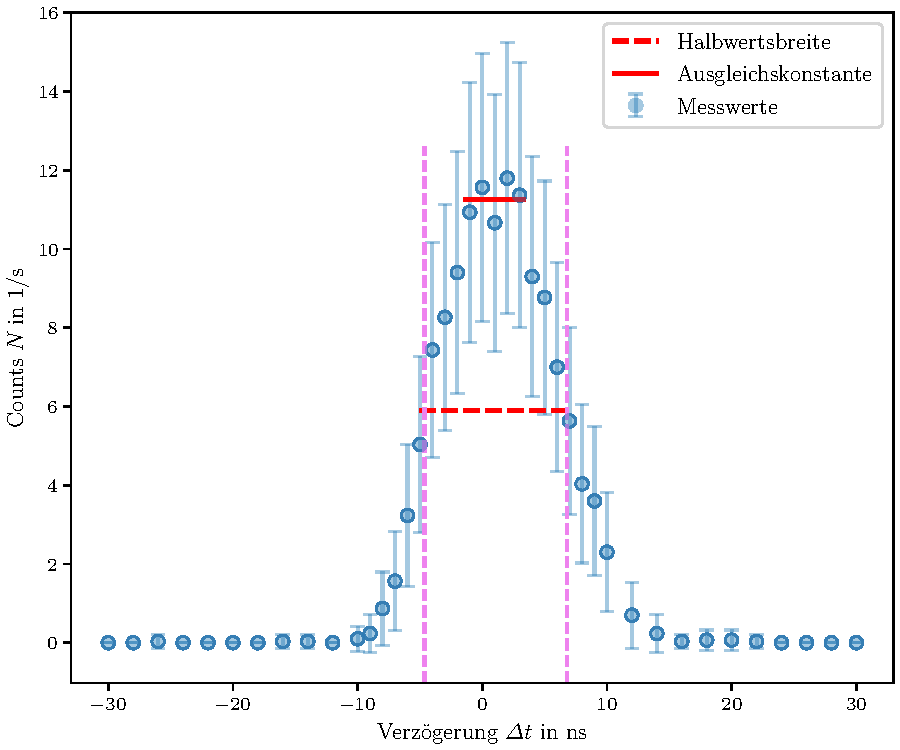
\includegraphics{Verzoegerung.pdf}
  \caption{Plot.}
  \label{fig:Verzoegerung}
\end{figure}

%Siehe \autoref{fig:plot}!